
\section{对齐选项}
\label{sec:pgfplots:sec:align}

\subsection{基本对齐}

对齐通过两种主要方式工作：一个要在其上绘制坐标轴的坐标，以及坐标轴内部一个要绘制在该特定坐标处的“锚点”。这种方法对每个 \Tikz{} 节点都很常见——而坐标轴不过是一个（特殊的）\Tikz{} 节点。坐标可以使用 |at| 键指定，而锚点可以使用 |anchor| 键指定。在大多数情况下，仅提供锚点就足够了——除非需要在同一图片环境中有多个坐标轴。

\begin{pgfplotskey}{at=\marg{coordinate expression}}
    为整个坐标轴图像指定一个位置。此选项的工作方式与 |\node[at=|\marg{coordinate expression}|]| 的 |at| 选项类似，参见~\cite{tikz}。常用语法为 |at={|\parg{x,y}|}|。

    其思想是提供一个 \meta{coordinate expression}，坐标轴将放置在该处。坐标轴的锚点将放置在 \meta{coordinate expression} 处。
\end{pgfplotskey}

\begin{pgfplotskey}{anchor=\marg{name} (initially south west)}
\label{option:anchor}
    选择使用 |at| 放置的坐标轴内部不同可能位置之一。|at| 键定义在嵌入图片中放置坐标轴的位置，|anchor| 键定义坐标轴的哪个点应由 `|at|' 定位。初始配置假定 |at={(0,0)}|。因此，|anchor=center| 会将坐标轴的中心放置在逻辑图片位置 $(0,0)$。类似地，|anchor=south west| 会将坐标轴的左下角定位在 $(0,0)$。

    对于熟悉 \Tikz{} 的用户：坐标轴实际上是一个非常特殊的节点，因此锚点的工作方式如~\cite{tikz}。

    锚点与图的水平或垂直对齐结合使用时很有用，参见下面的示例。

    有四组可用的锚点：位于坐标轴包围盒上的锚点、位于外部包围盒上的锚点，以及一个坐标在外部包围盒上、另一个坐标在坐标轴矩形某位置的锚点。最后，还可以在原点附近放置锚点。

    {%
    %\pgfplotsset{every picture/.append style={background rectangle/.style={help lines},show background rectangle}}%
    \pgfplotstableread{pgfplots.testplot}\plottable
    \def\plot{%
        \begin{axis}[
            width=5cm,
            name=test plot,
            xlabel=$x$,
            ylabel={$y$},% = \frac 12 \cdot x^3 - 4 x^2 -16 x$},
%            legend style={at={(1.03,1)},anchor=north west},
            legend pos=outer north east,
            title=A test plot.,
        ]
            \addplot table from{\plottable};
            %\addplot coordinates {(0,0) (1,1)};
            \addlegendentry{$f(x)$}
            \addplot [red] plot [id=gnuplot_ppp,domain=-40:40,samples=120] gnuplot{10000*sin(x/3)};
            \addlegendentry{$g(x)$}
        \end{axis}
    }%
    \def\showit#1#2{%
        %\node[show them,#2] at (test plot.#1) {(s.#1)};
        \node[pin=#2:(s.#1),fill=black,circle,scale=0.3] at (test plot.#1) {};
    }%
    \tikzstyle{every pin}=[opacity=0.5,fill=yellow,rectangle,rounded corners=3pt,font=\tiny]%
    %
    更详细地说，我们有位于坐标轴矩形（坐标轴周围的包围盒）上的锚点，\footnote{\PGFPlots{} v.1.3 之前的版本\emph{没有}使用坐标轴的包围盒，它们使用坐标轴坐标来定位这些锚点。这已被修复。如果你\emph{真的}想撤销此错误修复，参见 \texttt{\protect\pgfmanualpdfref{compat/anchors}{compat/anchors}}。}
    %
        \begin{center}
            \begin{tikzpicture}
                \plot
                \showit{north}{90}
                \showit{north west}{135}
                \showit{west}{180}
                \showit{south west}{225}
                \showit{south}{270}
                \showit{south east}{305}
                \showit{east}{0}
                \showit{north east}{45}
                \showit{center}{90}
            \end{tikzpicture}
        \end{center}
    %
    位于外部包围盒上的锚点，
    %
        \begin{center}
            \begin{tikzpicture}
                \plot
                \showit{outer north}{90}
                \showit{outer north west}{135}
                \showit{outer west}{180}
                \showit{outer south west}{225}
                \showit{outer south}{270}
                \showit{outer south east}{305}
                \showit{outer east}{0}
                \showit{outer north east}{45}
                \showit{outer center}{90}
            \end{tikzpicture}
        \end{center}
    %
    还有一些锚点，一个坐标在外部包围盒上，另一个在坐标轴矩形上，
    %
        \begin{center}
            \begin{tikzpicture}
                \plot
                {\pgfplotsset{every pin/.append style={pin distance=1cm}}%
                \showit{above north}{90}
                }%
                \showit{above north east}{45}
                \showit{right of north east}{0}
                \showit{right of east}{0}
                \showit{right of south east}{0}
                \showit{below south east}{-45}
                {\pgfplotsset{every pin/.append style={pin distance=1cm}}%
                \showit{below south}{-90}
                }%
                \showit{below south west}{-135}
                \showit{left of south west}{180}
                \showit{left of west}{180}
                \showit{left of north west}{180}
                \showit{above north west}{135}
            \end{tikzpicture}
        \end{center}
    %
    最后，我们有原点锚点，当坐标轴线穿过原点时特别有用，
    %
        \begin{center}
            \begin{tikzpicture}
                \begin{axis}[
                    name=test plot,
                    axis x line=center,
                    axis y line=center,
                    enlargelimits=false,
                    minor tick num=3,
                    tick style={semithick},
                    tick align=center,
                    xlabel=$x$,
                    ylabel=$y$,
                    every axis x label/.style={
                        at={(current axis.right of origin)},
                        anchor=north east,
                    },
                    every axis y label/.style={
                        at={(current axis.above origin)},
                        anchor=north east,
                    },
                    inner axis line style={->},
                ]
                    \addplot+ [domain=-2:5] {20*x};
                \end{axis}
                {\pgfplotsset{every pin/.append style={pin distance=1cm}}%
                \showit{above origin}{45}
                }%
                \showit{right of origin}{45}
                {\pgfplotsset{every pin/.append style={pin distance=1cm}}%
                \showit{below origin}{0}
                }%
                \showit{left of origin}{135}
                \showit{origin}{135}
            \end{tikzpicture}
        \end{center}

    \noindent 还有第五种锚点，它与坐标轴没有直接关系：你可以提供\emph{一个命名内部节点}的锚点。因此，你可以通过如下编写 |\node (|\meta{name}|) at |\parg{point coordinate}| {};| 来定义自己的锚点（使用下面描述的 |baseline| 选项）：
    %
\begin{codeexample}[]
Aligning at .......
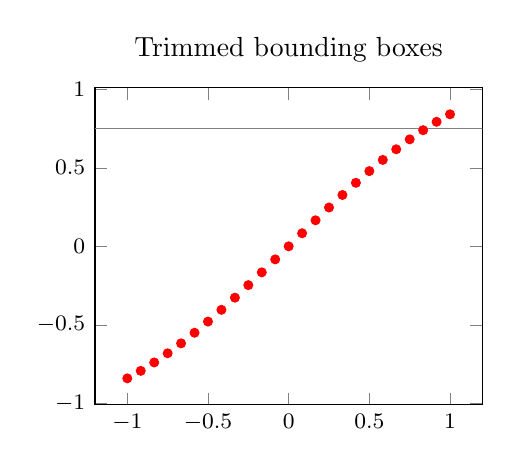
\begin{tikzpicture}[baseline]
\begin{axis}[small,anchor=aninnernode.center]
    \addplot {sin(deg(x))};
    \node
        [pin=-90:(aninnernode),fill=black,circle,scale=0.3]
            (aninnernode) at (-2,0.75) {};
    \draw [help lines] (-6,0.75) -- (6,0.75);
\end{axis}
\end{tikzpicture}
\end{codeexample}
    %
    \noindent 所发生的是一个节点被放置在 |(-2,0.75)|。请注意，选项 |[pin=...]| 仅用于显示 |\node|（pin 样式由 \PGFPlots{} 手册定义）。由于名称也可以使用 |name=|\meta{node's name} 来指定，并且由于任何 \PGFPlots{} 描述也是一个 |\node|，你可以在选定的坐标轴描述处对齐你的图：
    %
\begin{codeexample}[]
Aligning at .......
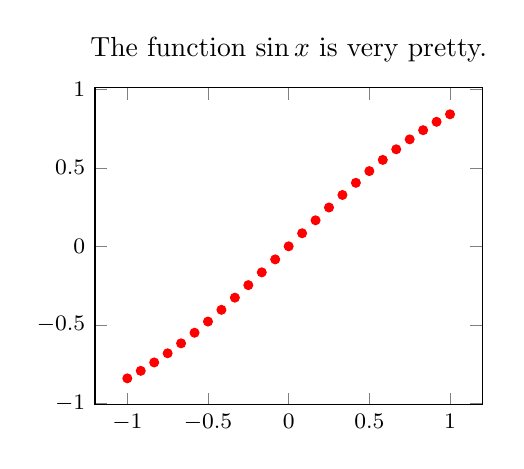
\begin{tikzpicture}[baseline]
\begin{axis}[
    small,
    title={The function $\sin x$ is very pretty.},
    title style={name=MyTitleNode},
    anchor=MyTitleNode.base,
]
    \addplot {sin(deg(x))};
\end{axis}
\end{tikzpicture}
\end{codeexample}

    默认值为 |anchor=south west|。你可以将锚点与 \Tikz{} 的 |baseline| 选项和/或
    |\begin{pgfinterruptbounding|\allowbreak|box}| 结合使用来执行对齐。


    \paragraph{备注：}

    坐标轴矩形上的每个锚点都对应于 Section~\ref{pgfplots:sec:axis:description:cs} 中描述的 |axis description cs| 中的一个坐标。这意味着第一组锚点实际上位于\emph{坐标轴周围的紧凑包围盒}上（没有任何刻度或描述）。即使在旋转或倾斜坐标系的情况下，|south west| 锚点也始终是此包围盒的左下角。\footnote{请注意，这仅对 1.3 之后的版本成立。}类似的说法也适用于其他锚点。

    }


    \subsection{使用 \texttt{baseline} 的垂直对齐}
    \label{sec:align}

    \begin{key}{/tikz/baseline}
        |baseline| 选项应作为参数提供给 |tikzpicture|。它配置 \Tikz{} 将图片位置 $y=0$ 移到嵌入文本的基线：
        %
\begin{codeexample}[width=3cm]
This is \tikz[baseline]\fill [red] (0,0) circle(3pt); a picture,
here \tikz[baseline]\fill [red] (0,10pt) circle(3pt); another one.
\end{codeexample}
        %
        \noindent 因此，|baseline| 选项允许对齐不同的 |tikzpicture|。坐标轴默认使用 |at={(0,0)}| 放置，而 |anchor| 键指定坐标轴的哪一部分放置在 |(0,0)|。因此，|baseline| 选项与 |anchor| 一起，允许将不同的坐标轴与嵌入文本对齐。

        默认坐标轴锚点为 |south west|，这意味着图片坐标 $(0,0)$ 是坐标轴的左下角。因此，\Tikz{} 选项 ``|baseline|'' 允许相邻图的垂直对齐：
        %
\begin{codeexample}[]
% 1. Unaligned:
\pgfplotsset{domain=-1:1}
\begin{tikzpicture}
    \begin{axis}[xlabel=A normal sized $x$ label]
        \addplot [smooth,blue,mark=*] {x^2};
    \end{axis}
\end{tikzpicture}%
    \hspace{0.15cm}
\begin{tikzpicture}
    \begin{axis}[xlabel={$\displaystyle \sum_{i=0}^N n_i $ }]
        \addplot [smooth,blue,mark=*] {x^2};
    \end{axis}
\end{tikzpicture}
\end{codeexample}

\begin{codeexample}[]
% 2. Aligned:
\pgfplotsset{domain=-1:1}
\begin{tikzpicture}[baseline]
    \begin{axis}[xlabel=A normal sized $x$ label]
        \addplot [smooth,blue,mark=*] {x^2};
    \end{axis}
\end{tikzpicture}%
    \hspace{0.15cm}
\begin{tikzpicture}[baseline]
    \begin{axis}[xlabel={$\displaystyle \sum_{i=0}^N n_i $ }]
        \addplot [smooth,blue,mark=*] {x^2};
    \end{axis}
\end{tikzpicture}
\end{codeexample}

        请注意，也可以写 |baseline=5cm|，在这种情况下，$y=\;$|5cm| 处的图像偏移将用作基线。
    \end{key}

    |baseline| 键与 |\begin{minipage}|\oarg{alignment} 或 |\begin{tabular}|\oarg{alignment} 相关：\meta{alignment} 告诉 \LaTeX{} |minipage| 或 |tabular| 的哪一部分应定位在基线上。因此，|baseline| 对图片做同样的事情（对 \meta{alignment} 有更多自由）。


    \subsection{水平对齐}
    \label{sec:halign}

    水平对齐可以通过两种方式完成：
    %
    \begin{enumerate}
        \item 使用具有缩小包围盒的独立 |tikzpicture| 环境，或
        \item 在单个 |tikzpicture| 环境中完成整个对齐。
    \end{enumerate}
    %
    第一种方法需要使用缩小的包围盒，并在 Section~\ref{sec:bb} 中讨论。

    第二种方法，即单个 |tikzpicture| 环境，使用 |at| 和 |anchor| 键来对齐图像的各个部分。例如，如果你将多个 |axis| 放入单个 |tikzpicture| 并使用 `|anchor|' 选项，你可以控制水平对齐：
    %
\message{'warning /pgfplots/warning/approx empty range enlarged' is expected here.^^J}%
\begin{codeexample}[]
\begin{tikzpicture}
\pgfplotsset{
  every axis/.append style={
    cycle list={
        {red,only marks,mark=*,
         mark options={fill=red,scale=0.8}},
        {black,only marks,mark=square*,
         mark options={fill=black,scale=0.8}}
    },
  },
}
\begin{axis}[
    width=4cm,scale only axis,
    name=main plot,
]
  \addplot file {plotdata/pgfplots_scatterdata1.dat};
  \addplot file {plotdata/pgfplots_scatterdata2.dat};
  \addplot [blue] coordinates {
      (0.093947,    -0.011481)
      (0.101957,    0.494273)
      (0.109967,    1.000027)
  };
\end{axis}
\begin{axis}[
    at={(main plot.below south west)},yshift=-0.1cm,
    anchor=north west,
    width=4cm,scale only axis,height=0.8cm,
    ytick=\empty,
]
    \addplot file
        {plotdata/pgfplots_scatterdata1_latent.dat};
    \addplot file
        {plotdata/pgfplots_scatterdata2_latent.dat};
\end{axis}
\end{tikzpicture}
\end{codeexample}

    这里，第二个坐标轴使用 |at={(main plot.below south west)}| 放置在第一个坐标轴下方。此外，它有 |yshift=-0.1cm| 以留出额外空间，并使用 |anchor=north west| 将左上角放置在指定位置。我们也可以不使用 |at={}| 结构，而使用具有更大负偏移的 |yshift|。


    \subsection{数组形式的对齐（子图）}
    \label{sec:pgfplots:arrayform}
        \index{Subplots}%
        \index{Alignment!Subplots}%
        \index{Alignment!Array}%
        \index{array!Array Alignment}%

    \pgfmanualpdflabel{\textbackslash matrix}{}%

    有时需要数组形式的多个对齐坐标轴。\PGFPlots{} 以多种方式支持此任务，如下所述。基本上有三种相关但不同的方法：
    %
    \begin{enumerate}
        \item 简单地将 |\begin{tikzpicture}...\end{tikzpicture}| 放入 \LaTeX{} 表格。这很直接；你对 |\includegraphics| 也会做同样的事情。

            除了 |\includegraphics| 之外，|baseline| 功能允许简单而有效的垂直对齐。此外，|trim left| 和 |trim right| 功能允许简单而有效的水平对齐（见下文）。
        \item 使用一个\emph{单个}图片，其中包含一个坐标轴数组，即类似

            |\begin{tikzpicture} \matrix{ |\meta{multiple axes}| }; \end{tikzpicture}| 的模式。

            这允许相当简单的对齐！可惜，由于 |\matrix| 的一个弱点，它需要对 |legend entries| 进行特殊处理。如果你使用 |external| 库（推荐），由于图片变大，会花费更多时间。
        \item 使用随 \PGFPlots{} 提供的 |groupplots| 库。它专门用于数组形式的坐标轴，当坐标轴密切相关时（例如它们共享坐标轴描述如 |xlabel| 甚至刻度标签）尤其强大。但请注意，在自动处理包围盒方面，其他方法更好。
    \end{enumerate}
    %
    |groupplots| 库在 Section~\ref{sec:group:plot} 中详细讨论。本节讨论另外两种方法。


    \paragraph{使用 \LaTeX{} 表格的数组对齐}

    其思想很简单：使用 \LaTeX{} 表格，并为每个单元格提供一个 |tikzpicture|。你可能熟悉这种对齐方式，也许是与 |\includegraphics| 一起使用。它对 \PGFPlots{} 以完全相同的方式工作。这种方法是最简单的，因为它不需要特殊知识。然而，它的缺点是更难控制图像\emph{内部}的位置（如不同大小的坐标轴描述）。

    强烈建议对每个单元格图片使用 |baseline| 选项，这会大大简化垂直对齐。如果你想要一个简单的解决方案来以数组形式放置独立坐标轴，并且你倾向于为每个坐标轴使用一个 |tikzpicture|，那么获得水平对齐的最简单也最有效的方式可能是 |trim left| 和 |trim right| 功能——或基于它们的样式：

    |trim axis left| 功能可用于将左侧的坐标轴描述排除在包围盒之外，|trim axis right| 可将右侧的坐标轴描述排除在包围盒之外。因此，对齐使用垂直坐标轴线完成。由于这两个键实际上修改了包围盒，它们在 Section~\ref{sec:bb}“包围盒限制”中记录。这里只是一个通过 |tabular|、|baseline| 和 |trim left|/|trim right| 功能进行数组对齐的小示例：
    %
\begin{codeexample}[vbox]
\pgfplotsset{
    small,
    title=Trimmed bounding boxes
}
\begin{center}
\begin{tabular}{rl}
    \begin{tikzpicture}[baseline,trim axis left]
        \begin{axis}
            \addplot {x};
        \end{axis}
    \end{tikzpicture}
        &
    \begin{tikzpicture}[baseline,trim axis right]
        \begin{axis}[
            ylabel={$f(x)=x^2$},
            yticklabel pos=upper,
            ylabel style={font=\Huge},
        ]
            \addplot {x^2};
        \end{axis}
    \end{tikzpicture}
        \\
    \begin{tikzpicture}[baseline,trim axis left]
        \begin{axis}[xlabel=$x$,xlabel style={font=\Huge}]
            \addplot {x^3};
        \end{axis}
    \end{tikzpicture}
        &
    \begin{tikzpicture}[baseline,trim axis right]
        \begin{axis}[yticklabel pos=upper]
            \addplot {x^4};
        \end{axis}
    \end{tikzpicture}
        \\
\end{tabular}
\end{center}
\end{codeexample}
    %
    \noindent 该示例有 $2 \times 2$ 个坐标轴。|baseline| 功能控制垂直对齐：下方坐标轴线始终在同一高度。|trim axis left| 键是一个样式，它告诉 \Tikz{} 修剪左坐标轴线左侧的所有内容。类似地，|trim axis right| 键不包括右坐标轴线右侧的图片部分。结合 |\begin{center}| 和 |yticklabel pos=upper| 键，我们得到正确的水平和垂直对齐，以及在左、右坐标轴线处的居中（不含描述）。

    一个很大的优势是这种对齐类型几乎不需要更改你的图片。因此，你可以相对简单地复制粘贴现有图片（\TeX{} 代码）。

    请注意，这种方法与图像 |external|ization 库完全兼容：每个图片单独导出，包围盒限制（和 |baseline| 偏移）存储在单独的 |.dpth| 文件中。水平对齐的 |trim left|/|trim right| 方法是缩小包围盒和图像外部化\emph{唯一}支持的方式。


    \paragraph{使用 \Tikz{} 矩阵的数组对齐}

    虽然可以使用（例如）|tabular| 结合上面讨论的垂直和水平对齐方法，但使用 \Tikz{} |matrix| 可能更好，因为它自动处理坐标轴描述的大小。

    \Tikz{} 矩阵是某种“图形”表格。它了解图片对齐的一切，并且在图形方面比 |tabular| 更灵活。其思想是将整个数组打包到一个\emph{单个}图片中。

    \Tikz{} 矩阵的完整文档超出了本手册的范围，详情请参见 \cite{tikz}。但我们在这里提供一个示例：
    %
\pgfmanualpdflabel{/tikz/matrix}{}%
\begin{codeexample}[]
\begin{tikzpicture}
        \pgfplotsset{small}
    \matrix {
        \begin{axis}
            \addplot {x};
        \end{axis}
           &
        % differently large labels are aligned automatically:
        \begin{axis}[ylabel={$f(x)=x^2$},ylabel style={font=\Huge}]
            \addplot {x^2};
        \end{axis}
            \\
        \begin{axis}[xlabel=$x$,xlabel style={font=\Huge}]
            \addplot {x^3};
        \end{axis}
            &
        \begin{axis}
            \addplot {x^4};
        \end{axis}
            \\
    };
\end{tikzpicture}
\end{codeexample}
    %
    \noindent 因此，矩阵是 |tikzpicture| 内部的一个图片元素。它的单元格像 tabular 中一样由 `|&|' 分隔（或者，如果 `|&|' 引起问题，则用 |\pgfmatrixnextcell|）。它的行由 `|\\|' 分隔。每个单元格使用单元格的锚点对齐。由于默认情况下坐标轴的锚点放置在左下角，上面的示例完全对齐，不需要任何包围盒修改——甚至标签也正确对齐。如果要使用另一个锚点，只需放置
    %
\begin{codeexample}[code only]
    \pgfplotsset{anchor=...}
\matrix {
    ...
};
\end{codeexample}
    %
    \noindent 在矩阵前面。这将对每个子图使用相同的配置。


    \paragraph{注意：}

    不幸的是，使用 |\matrix| 的数组对齐需要对图例给予特别的\emph{注意}。图例也是一个 |\matrix|，而 \Tikz{} 矩阵不能嵌套。你需要使用 |legend to name| 功能（或通过 |\label| 和 |\ref| 组装图例）来克服这个弱点（详情参见 Section~\ref{pgfplots:legend:labelref}）。


    \subsection{对齐杂项}

    \begin{predefinednode}{current axis}
        一个指向当前坐标轴或最后排版的坐标轴的节点。

        你可以在坐标轴描述中使用此节点，例如放置坐标轴标签或标题。


        \paragraph{备注：}

        如果你在坐标轴描述内部使用 |current axis|，“当前坐标轴”尚未完成。这意味着你\emph{不能}在坐标轴描述内部使用任何外部锚点。

        也可以在坐标轴内部的任何绘图或制图命令中使用 |current axis|（但不能使用外部锚点，因为处理绘图命令时这些尚未定义）。这种用法类似于 |axis description cs|。
    \end{predefinednode}
\end{pgfplotskey}
